% !TEX root = main.tex

\section{随机方法} % 7.1-7.3 (7.4-7.5)
假设给定多个变量$s_i$,其中每个变量数值都取两个离散值之一,记为$\pm 1$。
优化问题为确定$N$个$s_i$的合适取值,使下述代价函数或能量函数最小
\[E=-\frac{1}{2}\sum_{i,j=1}^N w_{ij}s_is_j\]
其中$w_{ij}$是对称的,取值可正可负。
\begin{figure}[H]
\centering
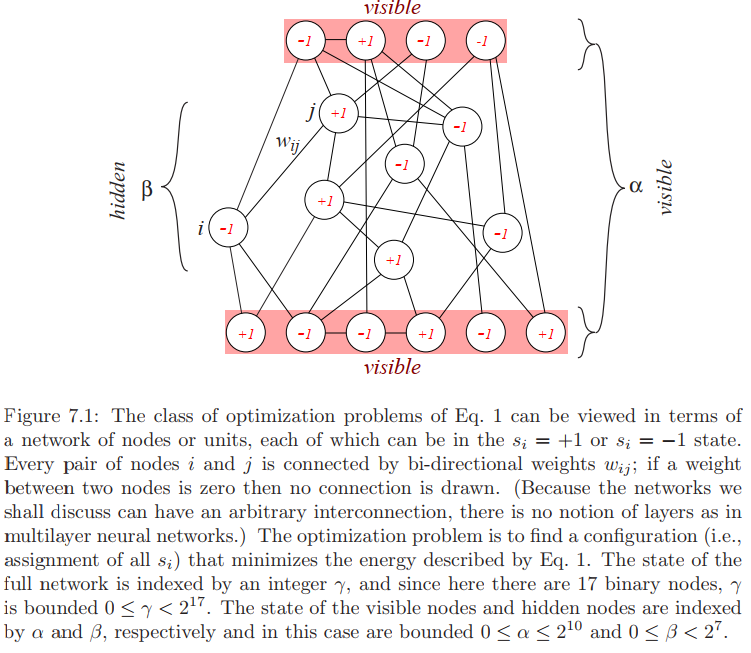
\includegraphics[width=0.9\linewidth]{fig/stochastic_opt_problem.png}
\end{figure}

\subsection{模拟退火}
一个系统具有能量$E_\gamma$通过下式给出
\[P(\gamma)=\frac{\ee^{-E_\gamma/T}}{Z(T)}\]
其中分子为Boltzmann因子,而$Z$是一个归一化常量/分配(partition)函数
\[Z(T)=\sum_{\gamma'}\ee^{-E_{\gamma'}/T}\]
为Boltzmann因子对所有构型的求和。

\begin{algorithm}[H]
\caption{模拟退火(Simulated Annealing)}
\begin{algorithmic}[2]
\State 将网络随机初始化,并设一个高的初始温度$T(1)$
\State 随机选择节点$i$,设其状态为$s_i=+1$,计算该构型下系统总能量$E_a$
\State 改变其道候选状态不$s_i=-1$,系统总能量为$E_b$
\If{$E_b<E_a$}
\State 接受此次状态改变
\Else
\State 以$\ee^{-\Delta E_{ab}/T}$概率接受改变,其中$\Delta E_{ab}=E_b-E_a$
\EndIf
\end{algorithmic}
\end{algorithm}
\begin{figure}[H]
\centering
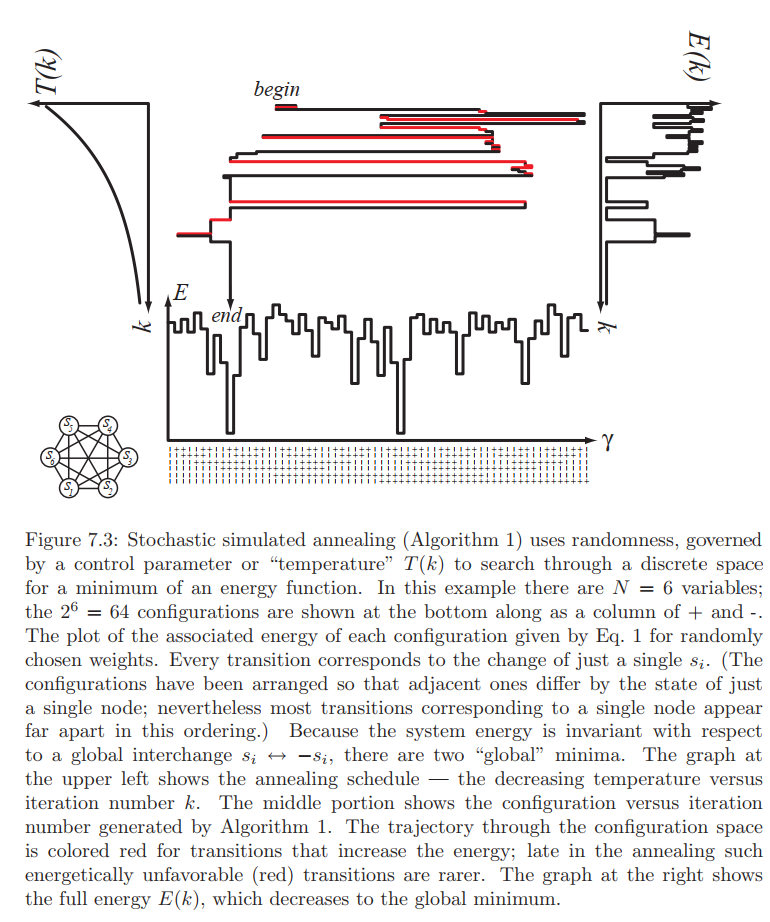
\includegraphics[width=0.8\linewidth]{fig/simulated_annealing.png}
\end{figure}

\subsection{Boltzmann学习}
\begin{figure}[H]
\centering
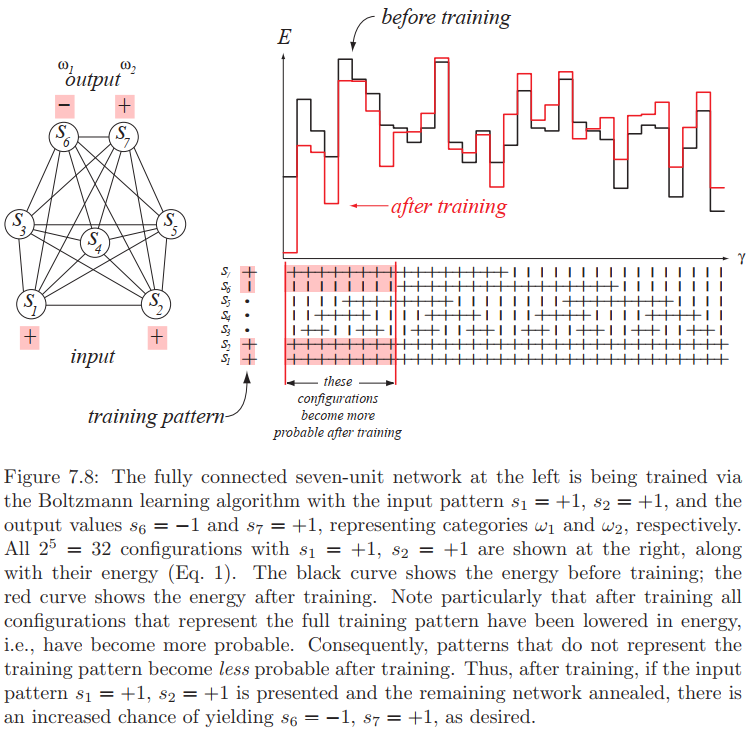
\includegraphics[width=0.8\linewidth]{fig/boltzmann_learning.png}
\end{figure}